\documentclass{Styles/llncs}
%\documentclass[12pt,letterpaper]{article}
\usepackage{times}

\usepackage[utf8x]{inputenc}
\usepackage[T1]{fontenc}

\usepackage{url}
\usepackage{amsmath}

\usepackage{graphicx}
\usepackage{caption}
\usepackage{subcaption}
\usepackage{subfig}
\usepackage{wrapfig}
\usepackage{multirow}
\usepackage{boxedminipage}
\usepackage{xspace}
\usepackage{listings}
\usepackage{listingsutf8}
\usepackage{verbatim}
\usepackage{parcolumns}
\usepackage{color}
\usepackage[usenames,dvipsnames,svgnames,table]{xcolor}
%Prevents floating item to "jump" between sections
\usepackage[section]{placeins}
\usepackage{booktabs}
\newcommand{\arevoir}[1]{#1}

\newcommand{\kaapi}{\textsc{\mbox{XKaapi}}\xspace}

\newcommand{\libXKOMP}{\textsc{libKOMP}\xspace}
\newcommand{\TG}[1]{{\color{red}\bfseries TG: #1}}
\newcommand{\FB}[1]{{\color{orange}\bfseries FB: #1}}
\newcommand{\PV}[1]{{\color{purple}\bfseries PV: #1}}

\usepackage{xcolor}
\usepackage{todonotes}
\usepackage[color,leftbars]{changebar}

\newcommand{\cfsect}[1]{(\textit{cf.} section~\ref{#1})}
\newcommand{\cfsectpage}[1]{(\textit{cf.} section~\ref{#1}, page~\pageref{#1})}
\providecommand{\figureref}[1]{\figname~\ref{#1}}
\providecommand{\cftab}[1]{(\textit{cf.} tableau~\ref{#1})}
\newcommand{\cmd}[1]{{\upshape\texttt{\symbol{"5C}#1}}}

\newenvironment{remarque}
{\description \item[Remarque:] \ \slshape}
{\enddescription}

\makeatletter
\newbox\sf@box
\newenvironment{SubFloat}[2][]%
  {\def\sf@one{#1}%
   \def\sf@two{#2}%
   \setbox\sf@box\hbox
     \bgroup}%
  { \egroup
   \ifx\@empty\sf@two\@empty\relax
     \def\sf@two{\@empty}
   \fi
   \ifx\@empty\sf@one\@empty\relax
     \subfloat[\sf@two]{\box\sf@box}%
   \else
     \subfloat[\sf@one][\sf@two]{\box\sf@box}%
   \fi}
\makeatother
\renewcommand\floatpagefraction{.9}
\renewcommand\topfraction{.9}
\renewcommand\bottomfraction{.9}
\renewcommand\textfraction{.1}
\setcounter{totalnumber}{50}
\setcounter{topnumber}{50}
\setcounter{bottomnumber}{50}
\renewcommand{\ttdefault}{pcr}
\lstset{
	tabsize=4,
%	frame=single,
	breaklines=true,
	basicstyle=\ttfamily,
	frame=tb,
	framerule=0.2pt,
%	frameround={tttt},
	showstringspaces=false,
	language=c,
%	linewidth=0.95\textwidth,
	keywordstyle=\color{black}\bfseries,
%	keywordstyle=\color{blue},
	commentstyle=\color{OliveGreen},
	stringstyle=\color{red}\itshape,
	inputencoding=utf8/latin1,
	numbers=left,
	numberstyle=\tiny,
	numbersep=5pt,
% OMP define
emph={\#,pragma, taskwait, omp, task, depend}, emphstyle=\color{RoyalBlue}\bfseries,
emph={[2]in,inout,out,cw,data,numa,thread}, emphstyle={[2]\color{BrickRed}\bfseries},
emph={[3]tied,untied,shared, firstprivate, private}, emphstyle={[3]\color{Gray}\bfseries},
emph={[4]lu0,fwd,bdiv,bmod}, emphstyle={[4]\color{DarkGreen}\bfseries},
emph={[5]affinity, omp_get_numa_num, omp_get_num_numas, omp_get_numa_from_data,omp_set_task_affinity}, emphstyle={[5]\color{DarkViolet}\bfseries},
    %moredelim=**[is][\only<3>{\color{red}}]{@}{@},
}
\lstdefinestyle{smaller}{basicstyle=\scriptsize\ttfamily}
\lstMakeShortInline|


%% For IFP algorithm
\usepackage[algoruled]{algorithm2e}
\usepackage{algorithmic}
\SetKwRepeat{Do}{do}{while}%

\usepackage{tikz}
\usetikzlibrary{arrows,patterns,plotmarks,shapes,snakes,er,3d,automata,backgrounds,topaths,trees,petri,mindmap}
\usetikzlibrary{patterns}
\usepgflibrary{patterns}
\usepackage{pgf}
\usepackage{pgfplots}



\newcommand{\benchs}{KASTORS }

\sloppy

\begin{document}

\title{TODO}
\author{
  Philippe Virouleau \and Adrien Roussel$^{*}$ \and François Broquedis \and Thierry Gautier \and Fabrice Rastello
 \vspace*{-1ex}}
\institute{
   Inria,
   Univ. Grenoble Alpes,  CNRS, Grenoble Institute of Technology, LIG, Grenoble, France
   LIP, ENS de Lyon, France\\
   $^{*}$ IFPEN, Rueil Malmaison\\
   \email{firstname.lastname@inria.fr}\\
   \email{thierry.gautier@inrialpes.fr}\\
}
\date{}
\maketitle

\begin{abstract}
  \vspace*{-5ex} TODO
\smallskip
  \noindent\textbf{Keywords:}
  \emph{
    OpenMP, task dependencies, affinity, runtime systems, NUMA
  }
\end{abstract}


\section{Introduction}

OpenMP has become a major standard to program parallel applications on a wide variety of parallel platforms ranging from desktop notebooks to high-end supercomputers. It provides keywords to express fine grain task-based parallelism that boost the applications performance and scalability on large scale shared memory machines. In particular, tasking in OpenMP helps the programmers parallelize applications with irregular workload, letting the runtime system in charge of performing load balancing through task scheduling in a dynamic way. However, very little support exists to express and to control the affinity between tasks and data on systems with a decentralized memory layout, like \emph{Non-Uniform Memory Architectures} (NUMA). On such systems, the memory is physically split into several banks, also called \emph{NUMA nodes}, which leads to different memory latencies and throughputs depending on the location of the memory bank a core is accessing data from. To get the most performance out of such architectures, OpenMP runtime systems thus need to be extended to make the task scheduler aware of both the underlying hardware and the relation that exists between a task and the data it accesses.

 We relate in this paper our experiences to reach high performance out of OpenMP numerical applications on 192-core NUMA machine. The recently-added \emph{places} concept in the OpenMP 4.0 specification provides ways of binding OpenMP parallel regions to user-defined partitions of the machine. This basically ends up binding the threads of the corresponding region to a set of cores. Thus, relying on the first-touch memory allocation policy as a portable solution to control memory binding, OpenMP places can help to control thread affinity with respect to the memory.
%Nevertheless, if this solution exists it remains cumbersome with inherent shortages: it does not ensure clarity in the program between computations and memory access; Design of library remains complex due to non-composable non functional properties; It does not provide robust solution when load is high unbalanced between threads of different parallel regions.
However, the concept behind OpenMP places needs to be extended to improve the performance of task-based applications, as tasks are most of the time scheduled over threads in a dynamic way according to a work-stealing execution model.  This is why the OpenMP \emph{Architecture Review Board} is currently discussing the introduction of a new \textit{affinity} feature to make the runtime system aware of the affinities between the tasks and the data they access.

In this paper, we present how we control task and data placement inside our OpenMP runtime system, implementing an \emph{affinity} clause which syntax is very close to the one currently discussed by the ARB. We also explain how we manage such information at runtime in order to improve the execution of task-based OpenMP programs on NUMA systems, with a particular focus on the scheduling data structure and the scheduling algorithm.

The contribution of this paper is threefold:
\begin{itemize}
\item We propose an OpenMP-friendly \emph{affinity} extension to the Clang-3.8 compiler able to express affinities between tasks and memory and pass this information along to the runtime system ;
\item We describe an extension to our task-based OpenMP runtime system to guide the scheduling of tasks according to such information to reach better performance on NUMA systems ;
\item We present some preliminary experimental results on running OpenMP benchmarks with tasks dependencies on a 192-core NUMA system, with and without using \emph{affinity}.
\end{itemize}

%Francois : je sais pas s'il faut le mettre dans l'intro ça.
%Some preliminary experimental results demonstrate the capacity to manage finer information such as handle by affinity of task and memory. By analyzing our experimental results, we note OpenMP depend tasks based programs, with assumption that all accessed memory regions are encoded in dependencies, can be automatically scheduled with the same level of performance without adding clause to specify affinity.

\PV{TODO, l'annonce du plan}
The remainder of this paper is organized as follows : blablabla.

\begin{figure}[t]
%\begin{center}
\begin{minipage}[c]{0.4\linewidth}
\begin{lstlisting}[frame=none,style=smaller,showlines=true,mathescape=true]{bicgstab}
 $\textbf{Compute}$ $r_0 = b - Ax_{0}$
 $r^{*}_{0}$ arbitrary
 $p_0 = r_0$
 $j=0$
 do {
	$\alpha_j = \dfrac{(r_j, r^*_0)}{(Ap_j,r^*_0)}$
	$s_j = r_j - \alpha_j A p_j$
	$ \omega_j = (As_j, s_j) / (As_j, As_j)$
	$x_{j+1} = x_j + \alpha_j p_j + \omega_j s_j$
	$r_{j+1} = s_j - \omega_j A s_j$
	$\beta_j = \dfrac{(r_{j+1},r^*_0)}{(r_j,r^*_0)} \times \dfrac{\alpha_j}{\omega_j}$
	$p_{j+1} = r_{j+1} + \beta_j ( p_j - \omega_j A p_j )$
	$j = j + 1$
 } while (!convergence)
\end{lstlisting}
\centerline{BiCGStab algorithm}
\end{minipage}\hfill
\begin{minipage}[c]{0.5\linewidth}
\begin{lstlisting}[frame=none,style=smaller,showlines=true,mathescape=true,firstnumber=1]{bicgstab}
$\textbf{Compute}$ $r_0 = b - Ax_{0}$

#pragma omp parallel
#pragma omp single
do {
	$t_j = Ap_j$
	$s_j = r_j - \alpha_j A p_j$
	$ \omega_j = (As_j, s_j) / (As_j, As_j)$
	$x_{j+1} = x_j + \alpha_j p_j + \omega_j s_j$
	$r_{j+1} = s_j - \omega_j A s_j$
	$\beta_j = \dfrac{(r_{j+1},r^*_0)}{(r_j,r^*_0)} \times \dfrac{\alpha_j}{\omega_j}$
	$p_{j+1} = r_{j+1} + \beta_j ( p_j - \omega_j A p_j )$
	$j = j + 1$
while (!convergence)
\end{lstlisting}
\centerline{Parallelization}
\end{minipage}
%\end{center}
\caption{BiCGStab Algorithm. Left: Mathematical formulation of the algorithm. Right: Sketch of the parallel program using a high level API interface.} \label{lst:bicgstab}
\end{figure}
\section{Motivation: examples where we need support}

The high memory throughput  of NUMA architectures~\cite{} have been introduced at the price of non uniformity in memory latency. On such architectures, accessing local memory access induces lower latency than accessing data on a remote memory bank. To get the most performance, computational units of work, like \emph{threads} and \emph{tasks}, should ideally only access local memory.

%Iteratif, creux, ça repose sur du matrix vecteur traité dans les résultats.

Many projects from the High Performance Computing research area deal with sparse linear solvers as fundamental building blocks.
Let us consider the BiCGStab~\cite{} algorithm, a classical method for solving sparse linear algebra systems. Listing of figure~\ref{lst:bicgstab} sketches the algorithm (left part). $A$ is the sparse matrix, $p_j$, $s_j$, $r_j$ are vectors. The algorithm is structured around a main loop that iterates until convergence. At each iteration, the algorithm performs global access to data in (sparse) matrix vector products ($A p_j$ at line 6 and $A s_j$ at line 8) as well in several dot products.

Parallelization of BiCGStab has been presented in several related works~\cite{,}. The algorithm of figure~\ref{lst:bicgstab} has been parallelized using one parallel region surrounding the main loop.

Another class of algorithms needing special care regarding data locality is the Stencil algorithm.
These algorithms consist of multiple timesteps during which every element of an
array is updated using the value of its neighbors. Figure~\ref{fig:eval-jacobi-before} shows
the base performances of our Jacobi kernel, a stencil algorithm, evaluated on a
192 cores NUMA architecture, with both Clang's OpenMP runtime and our OpenMP runtime \libXKOMP.
We can see that the performances of either
task-based version is very poor. The reason behind this is that tasks are not
scheduled close to their data, and we will discuss this in details in Section~\ref{sec:experiment}.


\begin{figure}[t]
  \centering
  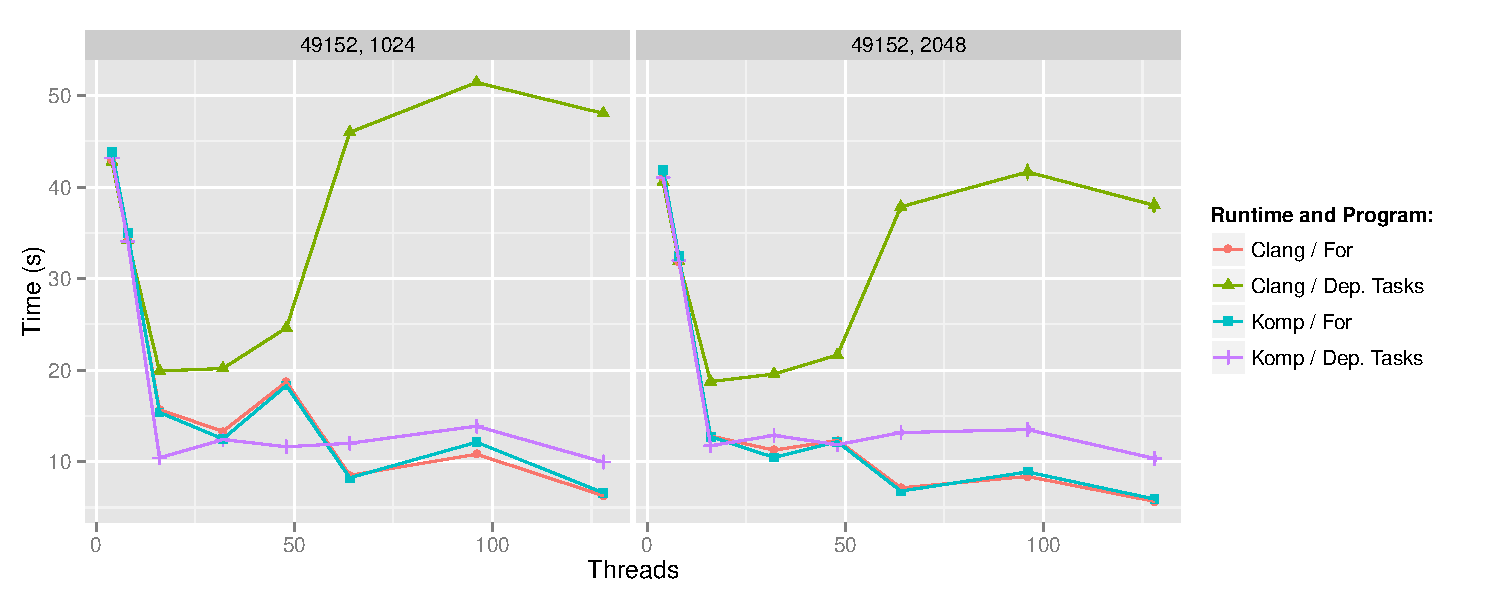
\includegraphics[scale=0.6]{graphs/jacobi_scale_iomp_komp.pdf}
  \caption{Jacobi's base performances}
\label{fig:eval-jacobi-before}
\end{figure}

\section{Extending OpenMP to support affinities}

In this section, we describe the details of our proposition, starting with the
language extension description, followed by our runtime extensions we implemented
to take advantage of this information.

\subsection{Modeling the architecture}

In order to express an affinity to a resource, one must first define how to identify these
resources within the current team.

The environment variables \verb/OMP_PLACES/ and \verb/OMP_PROC_BIND/ can already
be use to define a list of places mapped on the underlying architecture, and on which the program will be executed.

We suggest to use the same approach with the variable \verb/OMP_NUMA_PLACES/,
defining a list of NUMA nodes on which the program will be executed.

TODO en discuter !

\TG{Important ici}

Pour les bancs NUMA, il faut procéder de la même manière : 
OMP\_NUMA\_PLACES => ensemble de bancs NUMA à utiliser. A voir si ensemble d'ensemble ou non.
Dans le programme numaid i => ième banc numa dans OMP\_NUMA\_PLACES.
Si OMP\_NUMA\_PLACES pas définit => par défaut == ensemble des bancs NUMA.

\subsection{Extension of the OpenMP Task directive}

We propose an extension to precisely control the \emph{affinity} of a task with a specific part of the architecture hierarchy.

The two main components of NUMA architectures we consider in this work are cores and nodes. One of
the key to get performances out of NUMA architectures is to ensure tasks are
executing \emph{close} to their data.
Therefore we identified three different kinds of \emph{affinity} the programmer
may need to express, which are the following:
\begin{description}
    \item [affinity to a thread:]
      the runtime should try to schedule the task to be executed by a given thread.

    \item [affinity to a NUMA node:]
      the runtime should try to schedule the task on any of the threads bound to
      a given NUMA node.

    \item [affinity to a data:]
      once a task becomes ready for execution, the runtime should try to schedule it on any of the threads bound to the NUMA node on which the given data has been physically allocated.
\end{description}

Additionally, the programmer can specify if this affinity is \emph{strict}, which means the task \textbf{must} be executed on the given resource, or not. In the latter case, the task scheduler may decide to execute the task on a different resource, to perform load balancing for example.

Since this extension is aimed for the tasking construct, we implemented it as a new
clause for the OpenMP \emph{task} directive. The proposed syntax for the clause is the following:
\begin{lstlisting}
affinity([numa,thread,data]: expr[, strict])
\end{lstlisting}

If the \emph{expr} refers to an out-of-bounds resource, the value is taken modulo the amount of resources.
In the case of an affinity to a data, if the NUMA node associated to the data can't be determined, it defaults to the first NUMA node of the team.

\subsection{Extension of the OpenMP runtime API functions}
In order to dynamically get information about the current team hierarchy, we also propose
the following runtime API functions:
\begin{lstlisting}
TODO valide dans une région parallèle
Dans deux régions successives, meme nombre de threads, meme places => tu as le même ensemble de noeuds numa
//Get the number of NUMA nodes in the team
omp_get_num_nodes(void);
//Get the NUMA node the task is currently executed on
omp_get_node_num(void);
//Get the NUMA node the data has been allocated on
omp_get_node_from_data(void *ptr);
\end{lstlisting}

These functions allow to query information about the hardware topology. On machines without NUMA support we consider that all the threads are on a single NUMA node.

We also added the following runtime API function that mimics the \textit{affinity} clause:
\begin{lstlisting}
//Set the affinity information to the next created tasks
omp_set_task_affinity( 
     omp_affinitykind_t, uintptr_t ptr, int strict);
\end{lstlisting}
The scope of the function call is the next created task in the current \textit{task region}.
This function takes an \texttt{omp\_affinitykind\_t} value (either \texttt{omp\_affinity\_thread}, \texttt{omp\_affinity\_numa} or \texttt{omp\_affinity\_data}) to specify which kind of affinity control is applied. \texttt{value} is either an integer that represents an identifier to the NUMA node, an identifier to a thread or an address in the process address space used to select the affinity NUMA node \textbf{when} the task becomes ready for execution.

We implemented these extensions in the Clang compiler, based on the 3.8 version\footnote{https://github.com/viroulep/clang}; and we also added the corresponding entry points in Clang's OpenMP runtime\footnote{https://github.com/viroulep/openmp}.
\TG{Dire qu'ils ne sont réellement implémentés que dans libKOMP.}


\subsection{Extension of the task scheduler to support affinity}

We implemented extensions in the OpenMP runtime developed in our team, \libXKOMP~\cite{Durand2013,libkomp},
which is based on the \kaapi~\cite{Bleuse2014,parco2015} runtime system.
\kaapi is a task-based runtime system, using workstealing as a general scheduling strategy.
This section gives a a brief description of some of its key internal structures and mechanisms.

\subsubsection{The way \kaapi models the architecture.}
\kaapi sees the architecture topology as a hierarchy of \verb/locality domains/.
A \verb/locality domain/ is a list of tasks associated with a subset of the machine processing units.
\kaapi's locality domains are very similar to the notion of \emph{shepherd} introduced in \cite{DBLP:journals/ijhpca/OlivierPWSP12}, or ForestGOMP's \emph{runqueues}~\cite{BroFurGogWacNam10IJPP}.
\kaapi most of the time only considers two levels of domains : node-level domains,
which are bound to the set of processors contained in a NUMA node, and processor-level domains, which are bound to a single processor of the platform.
This way, at the processor level one \verb/locality domain/ is associated to each of the physical cores, and
at the NUMA node level one \verb/locality domain/ is associated to each of the NUMA nodes.


\subsubsection{The way \kaapi enables ready tasks and steals them.}

The scheduling framework in \kaapi~\cite{Bleuse2014,parco2015} relies on virtual functions
for \textit{selecting a victim} and \textit{selecting a place} to push a ready task.
When a processor becomes idle, the runtime system calls a function, called  \verb/WSselect/ for \emph{work-stealing select}, to browse the topology to find a locality domain from which stealing a task from the domain's task queue.
%There are many ways to do so, implemented in different \emph{selection strategies} called \verb/WSselect/, for \emph{work-stealing select} in the remaining of the paper.
%Once a place is selected, the processor will take a ready task from its queue.

\subsubsection{Implementation of the support for affinity}
We extended the set of internal control variables (ICV) with an \textit{affinity-var} property, and provided some runtime API functions to get and to set this ICV. As ICVs are inherited from the generating implicit task of the parallel region to each task this region generates, \textit{affinity-var} can be considered as a per-task variable. The variable is composed of two fields: an \texttt{omp\_affinitykind\_t} value and an integer large enough to encode a pointer.

%The scope of this \textit{affinity} ICV value is the task lifetime. until the next task generating construct in the OpenMP task region of the encountering thread~\cite{openmp40}\TG{Qui vérifie le vocabulaire "task region of the encountering thread" : tâche courante en cours d'exécution}. 

When a task construct using the \textit{affinity} clause is encountered, the runtime sets the appropriate kind of affinity and the integer value in the ICVs.
During task creation, these parameters will be set in the internal task descriptor.

When a task becomes ready to be executed, the function responsible for the \textit{selection of the place} to push
the task will look at the affinity and select the appropriate locality domain. The capacity to defer the evaluation of the affinity until the task becomes ready allows the runtime to rely on the \verb/get_mempolicy/ function to identify the NUMA node on which a data is allocated.

As described earlier, an affinity can be \emph{strict} or not. To implement this we used
a private queue per locality domain. If the affinity is strict, the task is pushed to the locality domain's private queue.
During the \textit{victim selection}, a thread may only steal from the locality domain's
public queue (in case of a locality domain attached to a NUMA node, every thread on this node can steal from the private queue).

\section{Examples of use and experimentation results}

\subsection{Implementation in benchmarks}

We looked into our Jacobi application from the KASTORS benchmark suite~\cite{virouleau:hal-01081974}.
The application is a 2D stencil computational kernel that is repeatedly applied until
convergence is detected. We used a blocked version of this algorithm.
We used both a \emph{dependent tasks} based implementation and a \emph{for} based implementation.
Each operation on a point of the matrix depends on its neighboring blocks,
therefore the blocks should be physically evenly distributed among the nodes,
and the computational tasks should be located close to these data.

Knowing the number of cores in the team, the matrix size and the block size, we computed a mapping
between multiple neighboring blocks and the different cores.

We used the affinity clause to achieve two goals:
\begin{itemize}
    \item first, to ensure the physical distribution of the data during initialization:
      in the dependent tasks version, each memory block is touched for the first time
      in the initialization task, therefore pinning the task to a thread ensures
      the memory will be physically allocated on its NUMA node.
      Listing~\ref{lst:init-aff} shows an example of the blocks initialization.
    \item second, to ensure tasks stay close to their dependencies during computation, by putting them on their block's thread.
      Listing~\ref{lst:compute-aff} shows an example use of affinity during computation.
\end{itemize}


We implemented both a strict affinity and a non-strict affinity version.


\begin{figure}[htbp]
\begin{lstlisting}[caption=Example of use of the affinity clause for initialization,frame=tlrb,style=smaller,label=lst:init-aff]{lst:init-aff}
for (j = 0; j < ny; j+= block_size)
  for (i = 0; i < nx; i+= block_size) {
    #pragma omp task firstprivate(i,j) private(ii,jj)\
       affinity(thread:GET_PARTITION(i, j, block_size, nx, ny), 1)
    {
      for (jj=j; jj<j+block_size; ++jj)
        for (ii=i; ii<i+block_size; ++ii) {
          if (ii == 0 || ii == nx - 1 || jj == 0 || jj == ny - 1)
            (*unew)[ii][jj] = (*f)[ii][jj];
          else
            (*unew)[ii][jj] = 0.0;
        }
    }
  }
\end{lstlisting}
\end{figure}

TODO virer un des deux

\begin{figure}[htbp]
\begin{lstlisting}[caption=Example of use of the affinity clause for computation,frame=tlrb,style=smaller,label=lst:compute-aff]{lst:compute-aff}
// Compute a new estimate.
for (int j = 0; j < ny; j += block_size) {
  for (int i = 0; i < nx; i += block_size) {
    int xdm1 = i == 0 ? 0 : block_size;
    int xdp1 = i == nx-block_size ? 0 : block_size;
    int ydp1 = j == ny-block_size ? 0 : block_size;
    int ydm1 = j == 0 ? 0 : block_size;
    #pragma omp task shared(u_, unew_) \
                     depend(out: unew[i: block_size][j: block_size]) \
                     depend(in: f[i: block_size][j: block_size], \
                                u[i: block_size][j: block_size], \
                                u[(i - xdm1): block_size][j: block_size], \
                                u[i: block_size][(j + ydp1): block_size], \
                                u[i: block_size][(j - ydm1): block_size], \
                                u[(i + xdp1): block_size][j: block_size]) \
                     affinity(thread:GET_PARTITION(i, j, block_size, nx, ny), 1)
    compute_estimate(i/block_size, j/block_size, u_, unew_, f_, dx, dy,
                     nx, ny, block_size);
  }
}
\end{lstlisting}
\end{figure}

\subsection{Experimental results}
\label{sec:experiment}

We compared several blocked versions of the application with both the Clang's OpenMP runtime
and the \kaapi runtime. The \textit{jacobi\_block\_for} version uses \emph{for} constructs during initialization and computation, while the \textit{jacobi\_block\_taskdep} version generates tasks with dependencies for initialization and computation. Each version comes with or without using the \emph{affinity} extension we propose. We refer to these enhanced versions as \textit{jacobi\_block\_for\_affinity} and \textit{jacobi\_block\_taskdep\_affinity}.

The initialization part of the \textit{jacobi\_block\_for\_affinity} uses tasks
instead of the regular \emph{for} construct, so that we could use the affinity clause.
The computation part of the algorithm has not been changed, there is no affinity
during the computation.

décrire choix des tailles+tailles de bloc

Matrix size and blocksizes have been chosen so that partitioning easily match
the number of threads up to 128.

\begin{figure}[t]
  \centering
  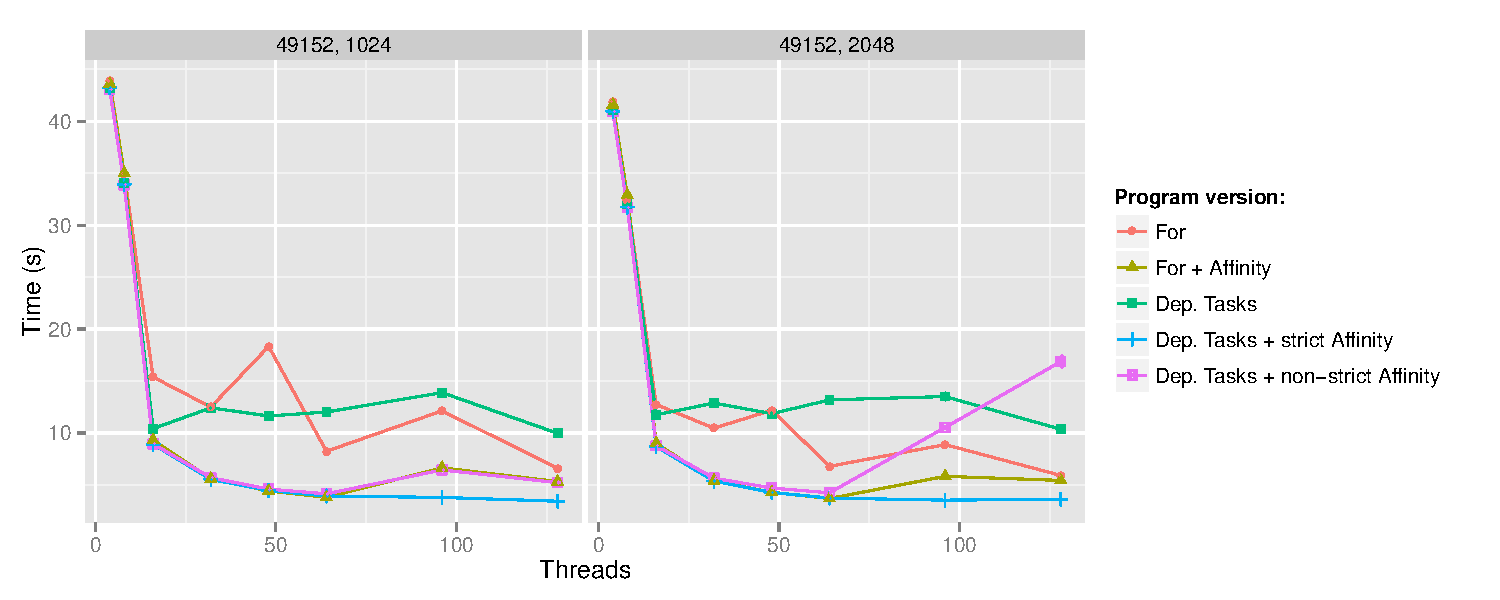
\includegraphics[scale=0.6]{graphs/jacobi_scale.pdf}
  \caption{Jacobi's performances overview using \libXKOMP, with a Matrix size of 49152, and blocksizes of 1024 or 2048}
\label{fig:eval-jacobi}
\end{figure}

conclusion: type d'application (stencil) tres dependant de la localisation de ses voisins
-> le cote strict permet de garantir que les taches ne bougent pas
-> ne pas mettre d'affinite/d'initialisation implique que les taches auront de gros temps d'acces a leurs donnees
-> régler le problème du block-for avec initialisation, si iterations dans le "bon" ordre ça se passe bien.

\subsection{Parallel linear algebra algorithms}

\subsubsection{Sparse Matrix Vector product (SpMV operation)}

In this section, we present two major algorithms of linear algebra. We split data following matrix graph partitioning techniques \cite{Saad:2003:IMS:829576} while using automatic graph partitioner like Metis~\cite{metis} tools. In such a decomposition, a matrix A is split in several sub-domains of several rows. A sub-graph is assigned to each partition, where internal nodes refers to block diagonal entries and off diagonal elements are stored in external matrix data structure. To ensure an efficient data distribution on numa nodes, all the local data structures to a partition are allocated in parallel. Vectors are split following row permutations and splitting dictated by graph partitioning, and local parts of the vectors are distributed too. Sparse matrix are stored in CSR format.

Let us consider now the operation $A \times X = Y$, where A is a sparse matrix, x is the input vector and b the output result. Considering the above data partitioning, the multiplication operation can be written as in figure~\ref{lst:spmv}.

\begin{figure}[t]
\begin{center}
\begin{minipage}[c]{0.9\linewidth}
\small{
}
\begin{lstlisting}[frame=none,style=smaller,showlines=true,mathescape=true,firstnumber=1]{spmv}
$\textbf{Compute} Y =  A\times X$
$A$ sparse matrix, see text for discussion
$X$ vectors, $X[i]$ sub vector associated to partition $i$
$Y$ same as $X$
/* omp parallel region outside the function */
for (i=0; i < $n_{partitions}$; ++i)
{
	#pragma omp task depend(in:X[i]) depend(out:Y[i]) \
		affinity(thread:i,0)
	/* store result in Y[i] */
	csr_mult( A.interior[i], X[i], Y[i]); 

	for (j=0; j < $A.neighbor\_of[i]$; ++j)
		#pragma omp task depend(in: X[j]) reduction(+: Y[i]) \
		     affinity( thread: i, 0)
		/* add result in Y[i]  */
		csr_mult_addin(A.interior[i][j], X[j], X[i]);
}
\end{lstlisting}
\end{minipage}\hfill
\end{center}
\caption{OpenMP SpMV Algorithm} \label{lst:spmv}
\end{figure}

Affinity are constrained by assigning the tasks to a thread following an owner compute rules: a task is mapped on the thread holding the output subvector $Y[i]$ (lines 8 and 14). 
%To avoid bus contention on the external copy for each sub-domain from their neighbors, we give a local copy of the vector $x$ to each numa node before SpMV computations for this test. TG: du fait des copies sans entrelacement par du calcul, il doit y avoir plus de contention
Each partition computations are encapsulated in an independent task, so the number of inserted tasks per SpMV operation is the number of partitions. 
In our experiment, $500$ iterates of SpMV operations are timed and the average times is reported in the figure~\ref{figs:spmv:3000} with an increasing number of threads $p$, where $p= {2,4,8,10,12,16,32,48,64,92,128,160,192}$. 
re the executions differs from the use of runtime systems. "XKaapi" stand for the use of XKaapi runtime system, and "Intel" the use of Intel runtime. For this experiment, we take matrices coming from the Finite Volume discretization of a 2D Laplace problem on several mesh sizes.  Reported graph is for mesh of size $2000 \times 2000$.

As we can see, for both executions the time spent to compute all the operations decreases. However, XKaapi runtime systems offers more powerful results because of the use of affinity clauses to place tasks on specific numa node where the output data is allocated to avoid massive data retrieving.
\TG{A reprendre: expliquer que intel runtime > increase because 2 numa nodes if p>8}
\TG{Pourquoi cela tend à diminuer ensuite ?}

\begin{figure}
  \centering
    \begin{tikzpicture}[scale=0.9]
      \begin{axis}[%ybar,
                   symbolic x coords = {2,4,8,10,12,14,16,32,48,64,92,128,160,192},
                   legend style = {area legend,legend pos = north east,},
                   xtick = data,
                   xticklabel style={/pgf/number format/1000 sep=},
                   width=1\textwidth,
                   xlabel=\textsc{cores},
                   ylabel=\textsc{time (seconds)}] 
        \addplot table[x=th,y=2000]{data/RuntimeSystems/iWomp/Spmv_omp.dat.csv};
        \addplot table[x=th,y=2000]{data/RuntimeSystems/iWomp/Spmv_kaapi.dat.csv};
        \legend{Intel,XKaapi};
      \end{axis}
    \end{tikzpicture}
    \caption{Mesh size: 2000x2000}
    \label{figs:spmv:2000}
\end{figure}



\section{Related Work}
\label{sec:related_work}

\TG{Related work de iwomp 2013. A reprendre ne garder que le gestion des queues etc.}\\

Many research projects have been carried out to improve execution of
OpenMP applications on NUMA machines.

The HPCTools group at the University of Houston has been working in
this area for a long time, proposing compile-time techniques that can
help improving memory affinity on hierarchical architectures like
distributed shared memory
platforms~\cite{Marowka:2004:OAD:1064428.1064431}. Huang et
al.~\cite{Huang-Chapman-locality-OpenMP} proposed OpenMP extensions to
deal with memory affinity on NUMA machines, like ways of explicitly
aligning tasks and data inside logical partitions of the architecture
called \textit{locations}.

TODO: préciser ici

While the proposed extension is interesting
to deal with regular memory-bound applications, it does not tackle
the problems induced by irregular workloads.

TODO paragraphe sur Andi

différence: modèle, travail niveau runtime et scheduling, pas de flexibilité niveau langage

Olivier et
al.~\cite{Olivier:2012:CMW:2388996.2389085}
introduced node-level queues of OpenMP tasks, called \textit{locality
  domains}, to ensure tasks and data locality on NUMA systems. The
runtime system does not maintain affinity information between tasks
and data during execution. Data placement is implicitly obtained
considering that the tasks access memory pages that were allocated
using the \textit{first-touch} allocation policy. The authors thus
ensure locality by always scheduling a task on the same locality
domain, preventing application programmers to experiment with other
memory bindings.

The INRIA Runtime group at the University of Bordeaux proposed the
ForestGOMP runtime system~\cite{BroFurGogWacNam10IJPP} that comes
with an API to express affinities between OpenMP parallel regions and
dynamically allocated data. ForestGOMP implements load balancing of
nested OpenMP parallel regions by moving branches of the corresponding
tree of user-level threads on a hierarchical way. Memory affinity
information is gathered at runtime and can be taken into account when
performing load balancing.


\section*{Acknowledgments}


This work is integrated and supported by the ELCI  project, a French FSN ("Fond pour la Société Numérique")
project that associates academic and industrial partners to design and provide software environment for very high performance
computing.
  \small \bibliographystyle{Styles/iplain}
%\nocite{*}
\bibliography{Bib/paper}

\end{document}
